\chapter{面向三轮对话的情感识别}
\label{cha:exp_context_emo}

\section{本章引论}

情感识别是意图识别中的核心课题之一,它尝试理解人们对特定对象如人物、机构、产品、服务等的情感倾向。虽然后自然语言处理领域已经有很长一段研究历史,但截至2000年为止针对人物情感和想法的研究甚少\cite{liu2012sentiment},而在2000年后情感识别开始受到关注,其中有以下几个的原因。首先是在各个领域出现了相关需求,商业上的需求间接导致资金支持的增加,基于情感识别的应用也因此得以发展,这些都为情感识别带来了研究动力。其次是数据的支持,在互联网出现前数据的收集普遍要透过人工完成,而在2000年后互联网逐渐普及,社交媒体的使用使得可供分析的数据远超于以前,数据的收集也更加便捷,这为研究提供了充足的数据基础。

面向文本的情感识别存在一些先天的难点。首先是一词多义,譬如在中文里“算账”有计算法资金收支或结余的意思,有引伸义为吃亏之后与人争执较量,又譬如在英文里“suck”有吸取或吸入物的意思,而在俚语中则有使人厌恶的意思,以上两个例子都是一个词可以在不同场景下表现中性和负性两种情感,这在情感识别中会导致混淆。其次是明显情感极性的词和发言者的情感无关,譬如“我想要挑一台好的电脑”,这里“好”有明显正向的词,但和发言者的情感无关,原句的情感应偏向于中性。第三是不带情感但包含情感极性的词组,譬如“打印机又卡纸了”的字面意思是偏中性的,但根据具体场景的经验,我们能猜想到发言者可能处于不耐烦的状态,间接表达的是负向的情感。最后是前面提到的反讽的修辞使用,透过表面上表现为正性的语句表达负性的情感。特别地,这些情况即使由人工识别也有可能会被混淆。

为了缓解在句子内部存在二义的问题,一些研究考虑引入上下文来提供辅助信息。譬如Zahiri和Choi\cite{Zahiri2017Emotion}在研究电影剧剧本情感识别时,就引入了前后的发言作为上下文信息来建模。而国际比赛SemEval-2019的任务三\cite{SemEval2019Task3}则是旨在促进引入上下文背景的文本情感识别研究,比赛要求参赛者开发一个情感识别系统,对三轮对话中最后一轮发言表达的情感进行分类,给定的四个情感类别包括:开心、悲伤、愤怒、其他。本章节中我们将基于SemEval-2019的任务三进行实验,采用比赛组织者提供的训练数据和测试数据,并透过和其他参赛系统进行比较来评估我们提出的框架的性能。

本章的内容安排如下。在章节\ref{sec:exp_context_emo_format}中,我们会基于章节\ref{sec:global_problem_analysis}首先给出当前问题的形式化表示。在章节\ref{sec:exp_context_emo_data}中我们再对具体实验数据进行观察,分析给定数据集中各个情感类别的分布情况以及其文本特性。在章节\ref{sec:exp_context_emo_framework}中,我们会基于章节\ref{sec:global_framework}的框架给出我们对当前问题的系统框架。最后在章节\ref{sec:exp_context_emo_exp}给出实验的细节,以及对实验结果进行分析。

\section{形式化表示}
\label{sec:exp_context_emo_format}

在本章中,我们要研究三轮对话的情感识别。给定一个情感类别集合$C$,对于一个三轮对话的集合$S$,其中任意一个样本$s$可以表示为一个三元组$<t^1, t^2, t^3>$对应三段文本,其中最后一轮发言$t^3$是被识别情感的主体,上下文$b=<t^1, t^2>$是$t^3$的背景信息。假设$t^3$在背景$b$下属于唯一一种情感倾向$c \in C$。又给定一个词集合$W$,对任意一轮的文本$t^j, j=1,2,3$,经过文本预处理后可以表示为一个长度为$L^j$的词序列 $w^j = <w^j_1, w^j_2, ..., w^j_{L^j}>, w^j_i \in W, i \in [1, L^j]$。那么我们的目标是找出一个映射关系$F_C$,使得$c=F_C(w^3, <w^1, w^2>)$。

\section{数据观察}
\label{sec:exp_context_emo_data}

我们的实验完全采用SemEval-2019的任务三比赛组织者提供的数据集,其中每个样本对应一个三轮对话以及第三轮发言的情感标签,第一轮为用户甲的发言(以下简称为A1),第二轮为用户乙对第一轮的回复(以下简称为B),第三轮为用户甲对第二轮中用户乙的回复(以下简称为A2)。情感标签对应四个情感类别中的其中一种:开心、悲伤、愤怒、其他。表\ref{tab:semeval_2019_task3_data}显示数据集各类别样本数量分布,表\ref{tab:semeval_2019_task3_sample}。

\begin{table}[htb]
  \centering
  \begin{minipage}[t]{0.8\linewidth}
  \caption{情感识别各类别样本数量分布}
  \label{tab:semeval_2019_task3_data}
    \begin{tabularx}{\linewidth}{X|XXXX}
    \toprule[1.5pt]
    数据集 & 其他 & 开心 & 悲伤 & 愤怒 \\  
    \hline
    训练集 & 14948 & 4243 & 5463 & 5506 \\
    验证集 & 2338 & 142 & 125 & 150 \\
    测试集 & 4677 & 284 & 250 & 298 \\
    \bottomrule[1.5pt]
    \end{tabularx}
  \end{minipage}
\end{table}

\begin{table}[htb]
  \centering
  \begin{minipage}[t]{\linewidth}
  \caption{情感识别各类别样例}
  \label{tab:semeval_2019_task3_sample}
    \begin{tabularx}{\linewidth}{l|XXX}
    \toprule[1.5pt]
    \small 情感类别 & 第一轮 & 第二轮 & 第三轮 \\
    \hline
    \small 开心 & live in uttra khand & ohh nice! love that place!∧.∧ & :):) \\
    \small 悲伤 & Not coz of you & why? Tell me & :( My girlfriend left me \\
    \small 愤怒 & He is over me & so YOU say & I just hate him \\  
    \small 其他 & degreee & what degree \& where? & sryyy i really got to goo\\
    \bottomrule[1.5pt]
    \end{tabularx}
  \end{minipage}
\end{table}

可见在训练集上四个类别的样本分布约为3:1:1:1 ,而在验证集和测试集上四个类别的样本分布约为22:1:1:1 。在测试集上“其他”一类的样本远高于其他三个类别,和训练集相比其样本比例也相对较高,而另外三个类别的样本数量则大致相同。

另外在官方的最终测试阶段,训练集和验证集均已公布情感标注并且可用于模型训练,因此我们在模型训练时结合了这个两个数据集,而在后续内容我们以训练集代表这个结合后的数据集。

\subsection{文本长度}

我们首先对数据集的文本经过简单分词后统计各个类别的样本中词数量的分布,以下简称为文本长度。表\ref{fig:context_emo_train_class_len}显示在训练集上各情感类别的样本在每轮发言的文本长度分布,可以看出在每一轮的发言中,不同类别样本的文本长度分布大致相同。虽然第一轮和第三轮的样本中最长的文本分别达到146个词和74个词,各轮样本的文本长度大部分在22个词以内,约为第\ref{cha:exp_irony_det}章中样本长度的一半。

\begin{figure}[h]
  \centering%

  \begin{minipage}{\linewidth}

  \subcaptionbox{第一轮\label{fig:context_emo_train_class_len_0}} %[3cm] 
    {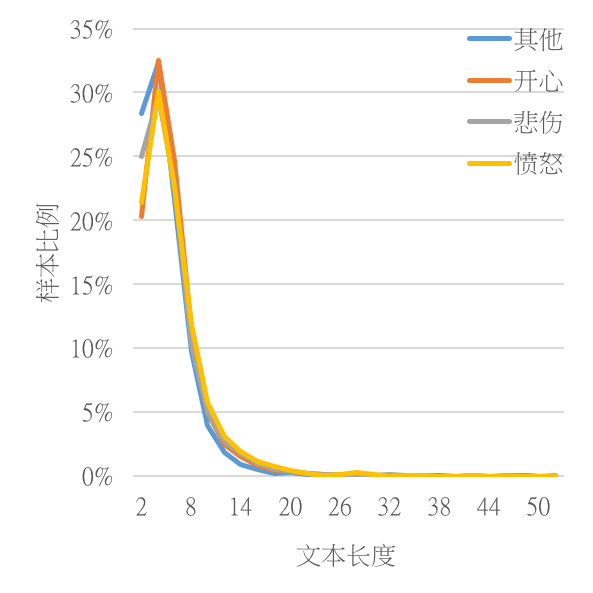
\includegraphics[height=8cm]{img/semeval2019_task3_train_0_class_len.png}}%
  %\hspace{em}%
  \subcaptionbox{第二轮\label{fig:context_emo_train_class_len_1}}
      {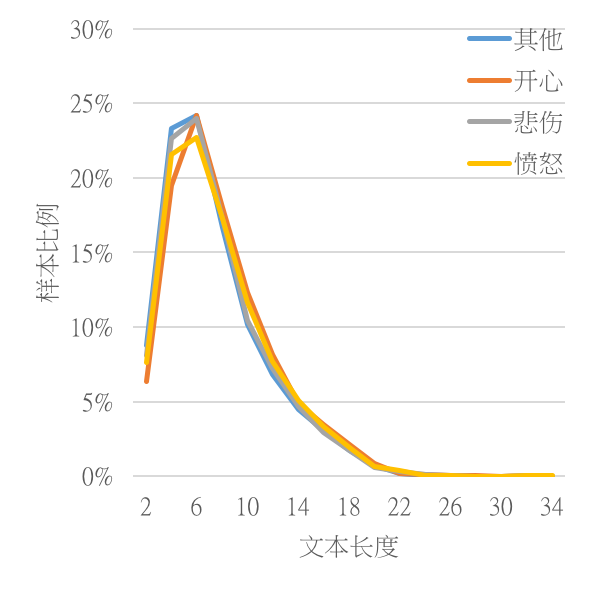
\includegraphics[height=8cm]{img/semeval2019_task3_train_1_class_len.png}}

  \end{minipage}
  \vspace{0.5cm} 

  \subcaptionbox{第三轮\label{fig:context_emo_train_class_len_2}}
      {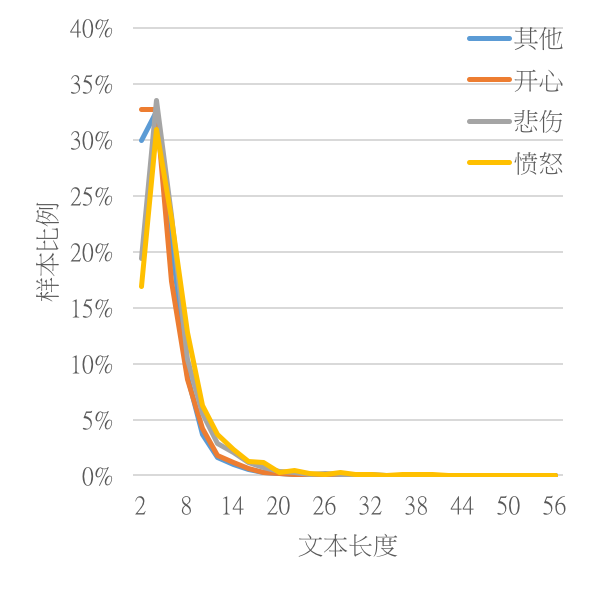
\includegraphics[height=8cm]{img/semeval2019_task3_train_2_class_len.png}}

  \caption{训练集上各情感类别的样本在每轮发言的文本长度分布}

  \label{fig:context_emo_train_class_len}
\end{figure}

\subsection{文本特征}
\label{ssec:exp_context_emo_data_text}

对于比赛中提供的数据集,比赛组织者并没有给出数据的具体来源,但经过人工观察后我们可以发现一些社交网络上常见的文本特征,其中出现频率较高的模式如下:

\begin{itemize}

\item 大量的缩略词使用,如“u”代替“you”,“y”代替“why”,“im”代替“I am”。和微博以及讨论区等场景相比,可以认为在聊天场景下,用户会倾向于更快速的响应,使用缩略语减少需要输入的字符从而加快了回覆消息的速度。

\item 出现在句子最前或最后的表情符,其中包括Unicode定义表情符和由标点符号组成的表情符两类。

\item 一些在社交媒体平台上常见的、有别于正规英语的用法,如拼写错误、全大写字母的单词等,可以参考章节\ref{sec:text_preprocess}描述的例子。

\end{itemize}

\subsection{各轮发言间的情感信息}
\label{ssec:exp_context_emo_multi_turn_analyse}

为了结合多轮发言的信息来预测最后一轮发言的情感,我们需要观察各轮发言是对最后一轮发言的情感有提示作用,如果有的话应该如何利用这些提示信息来进行识别,并将此机制体现在分类器模型的设计当中。以下我们将采用数据集中的具体例子解释我们对语料的观察和分析。

首先,对于三轮发言中两个用户的情感,我们发现用户甲和用户乙表达的情感可能截然不同,参考以下例子:

\makebox[4 cm]{(第一轮)用户甲:} yes yay fun\par
\makebox[4 cm]{(第二轮)用户乙:} are not you joining us? :( \par
\makebox[4 cm]{(第三轮)用户甲:} yes\par

用户甲在最后一轮发言的情感标签为“开心”,而第一轮发言在字面意思上同样偏向正面。而对于用户乙在第二轮的发言,根据上下文意思和最后文本末尾的“:(”,我们可以推断用户乙的情感为“伤心”。可见三轮对话中两个用户的表达的情感可能不同甚至矛盾,因此用户甲的发言和用户乙的发言对识别第三轮发言的情感应起着不同的作用,第二轮中用户乙的发言甚至没有提示的作用。

另外对于用户甲,我们发现他在第一轮和第三轮中表达的情感也有可能不同,参考以下例子:

\makebox[4 cm]{(第一轮)用户甲:} not fine\par
\makebox[4 cm]{(第二轮)用户乙:} why? :'o \par
\makebox[4 cm]{(第三轮)用户甲:} tomorrow lab exam\par

用户甲在最后一轮发言的情感标签为“悲伤”,而在字面意思上,最后一轮发言的情感偏中性,只是在陈述“明天有考试”的事情,“悲伤”的情感提示主要来自用户甲在第一轮中表示自己的情况“不太好”,第三轮发言在解释“不太好”的原因。基于此例子可以认为,同为用户甲发言的第一轮在某此情况下对识别第三轮发言的情感起着决定性作用。再观察下面的例子:

\makebox[4 cm]{(第一轮)用户甲:} ohh sorry\par
\makebox[4 cm]{(第二轮)用户乙:} do not worry, you are not the first \par
\makebox[4 cm]{(第三轮)用户甲:} glad to hear\par

用户甲在最后一轮发言的情感标签为“开心”,对于用户甲在第一轮发言表达的情感,结合用户乙在第二轮的发言,可以认为用户甲在第一轮发言中表示对用户乙的同情,这与“开心”为不同的情感,而在用户乙发言后,用户甲情感因为用户乙说的话而转换成“开心”。可见用户甲在第一轮和第三轮中表达的情感有可能不同,这种情感的转变可能由用户乙的发言造成,但无论具体原因是什么,用户甲在第一轮和第三轮中的发言对识别第三轮发言的情感应起着不同的作用。

再者,我们发现用户甲在第三轮发言中可能出现多于一种情感,参考以下例子:

\makebox[4 cm]{(第一轮)用户甲:} 
\includegraphics[height=1.5\fontcharht\font`\B]{img/emoji/laugh.png} yes yes \par
\makebox[4 cm]{(第二轮)用户乙:} :3 you seem like a happy person \par
\makebox[4 cm]{(第三轮)用户甲:} yes 
\includegraphics[height=1.5\fontcharht\font`\B]{img/emoji/lol.png} happy outside, 
\includegraphics[height=1.5\fontcharht\font`\B]{img/emoji/frown.png} sad inside \par

用户甲在最后一轮发言的情感标签为“悲伤”,而在文本上,第三轮发言的前半表现为正面情感,后半表现为负表情感,前后的情感出现了转变。对于当第三轮发言中出现两种情感时情感标签以何者为准,比赛组织者并没有给出细节的说明。

最后总给我们对语料中的样本进行的人工观察,我们发现三轮发言对识别第三轮发言的情感应起着不同的作用。当第三轮发言有明显的情感表达,我们可以无视前两轮发言的信息得出识别结果。当第三轮发言表达的情感较隐晦或偏中性,需要参考同为用户甲发言的第一轮的信息。第二轮发言的信息对情感识别没有明显的辅助作用,有待实验中进一步确认。

\section{框架设计}
\label{sec:exp_context_emo_framework}

我们提出的识别系统包含了三组分类器,分别面向不同的子分类问题,并依次经过三次投票结合各组分类器的预测结果来得出最终的预测结果。第一组分类器由$N_1$个四类分类器组成,对应原问题的四个类别:“开心”、“悲伤”、“愤怒”和“其他”。第二组分类器由$N_2$个三类分类器组成,用于区分“开心”、“悲伤”和“愤怒”三类。第二组分类器由$N_3$个二类分类器组成,用于区分“其他”和不是“其他”两类(即把“开心”、“悲伤”、“愤怒”视为一个情感类别)。

对于一条待识别的微博,决策过程如下:

\begin{itemize}

\item 首先由第一组分类器内部进行多数投票得出$Label^{1}_{MV}$作为第一轮的预测结果$Label_{I}$。为方便阅读,以下将对一组样本的第一轮预测结果称为中间结果I。

\item 第二步,由第二组分类器投票进行多数投票得出预测结果$Label^{2}_{MV}$,若超过$thr_{2}$分类器投票投给$Label^{2}_{MV}$且第一轮的预测结果$Label_{I}$为“其他”以外的三种情感类别之一,则把预测结果修改为$Label^{2}_{MV}$,否则保持不变,以此得出第二轮的预测结果$Label_{II}$。为方便阅读,以下将对一组样本的第二轮预测结果称为中间结果II。

\item 最后步,由第三组分类器分别得出预测结果,若超过$thr_{3}$分类器投票投给“其他”且第二轮的预测结果$Label_{II}$不是“其他”,则把预测结果修改为“其他”,否则保持不变,以此得出第三轮的预测结果$Label_{III}$,同时作为整个系统对该三轮对话的最终情感识别结果。

\end{itemize}

整个决策过程可以分成两大部分。第一部分是初步完成对第三轮发言的四分类情感识别,作为后续决策的基础,对应上述三步决策中的第一步。第二部分是基于第一部分的初步识别结果进行修正,对应上述三步决策中的后两步。第二步只关注于对“开心”、“悲伤”和“愤怒”三类的识别进行调整,因此对第一轮中被识别为“其他”的样本不作改动。而第三步则是关注于对“其他”一类的召回,这受启发于样本的数据分布的不均匀。在原比赛中,组识者在最后的测试阶段虽然没有给出各个样本的真实标签,但指出了“其他”、“开心”、“悲伤”和“愤怒”四个类别在测试集上的样本比例约为88:4:4:4 ,而在训练集上的比例约为55:15:15:15 ,“其他”的样本占比在测试集上要远高于训练集。因为针对性提高“其他”一类的召回有助于提高系统在测试集上的性能。值得注意的是虽然在大部分情况下,我们无法得出应用场景的真实标签,但可以透过社会学和统计学等手段评估应用场景上各类样本的分布。而为了模型训练,我们可以人为控制训练数据上各类样本的比例。在了解到训练集和测试集上样本数据分布存在差异的情况下,提高系统对个别类别的识别倾向,其中存在其合理性。另外,虽然此框架中第二部分的设计和章节\ref{sec:exp_irony_det_framework}中的有所不同,但同样引入了可信度的概念,第二步和第三步都只在足够多个分类器给出相同结果时才对上一轮的结果进行修正。

\begin{figure}[H]
  \centering
  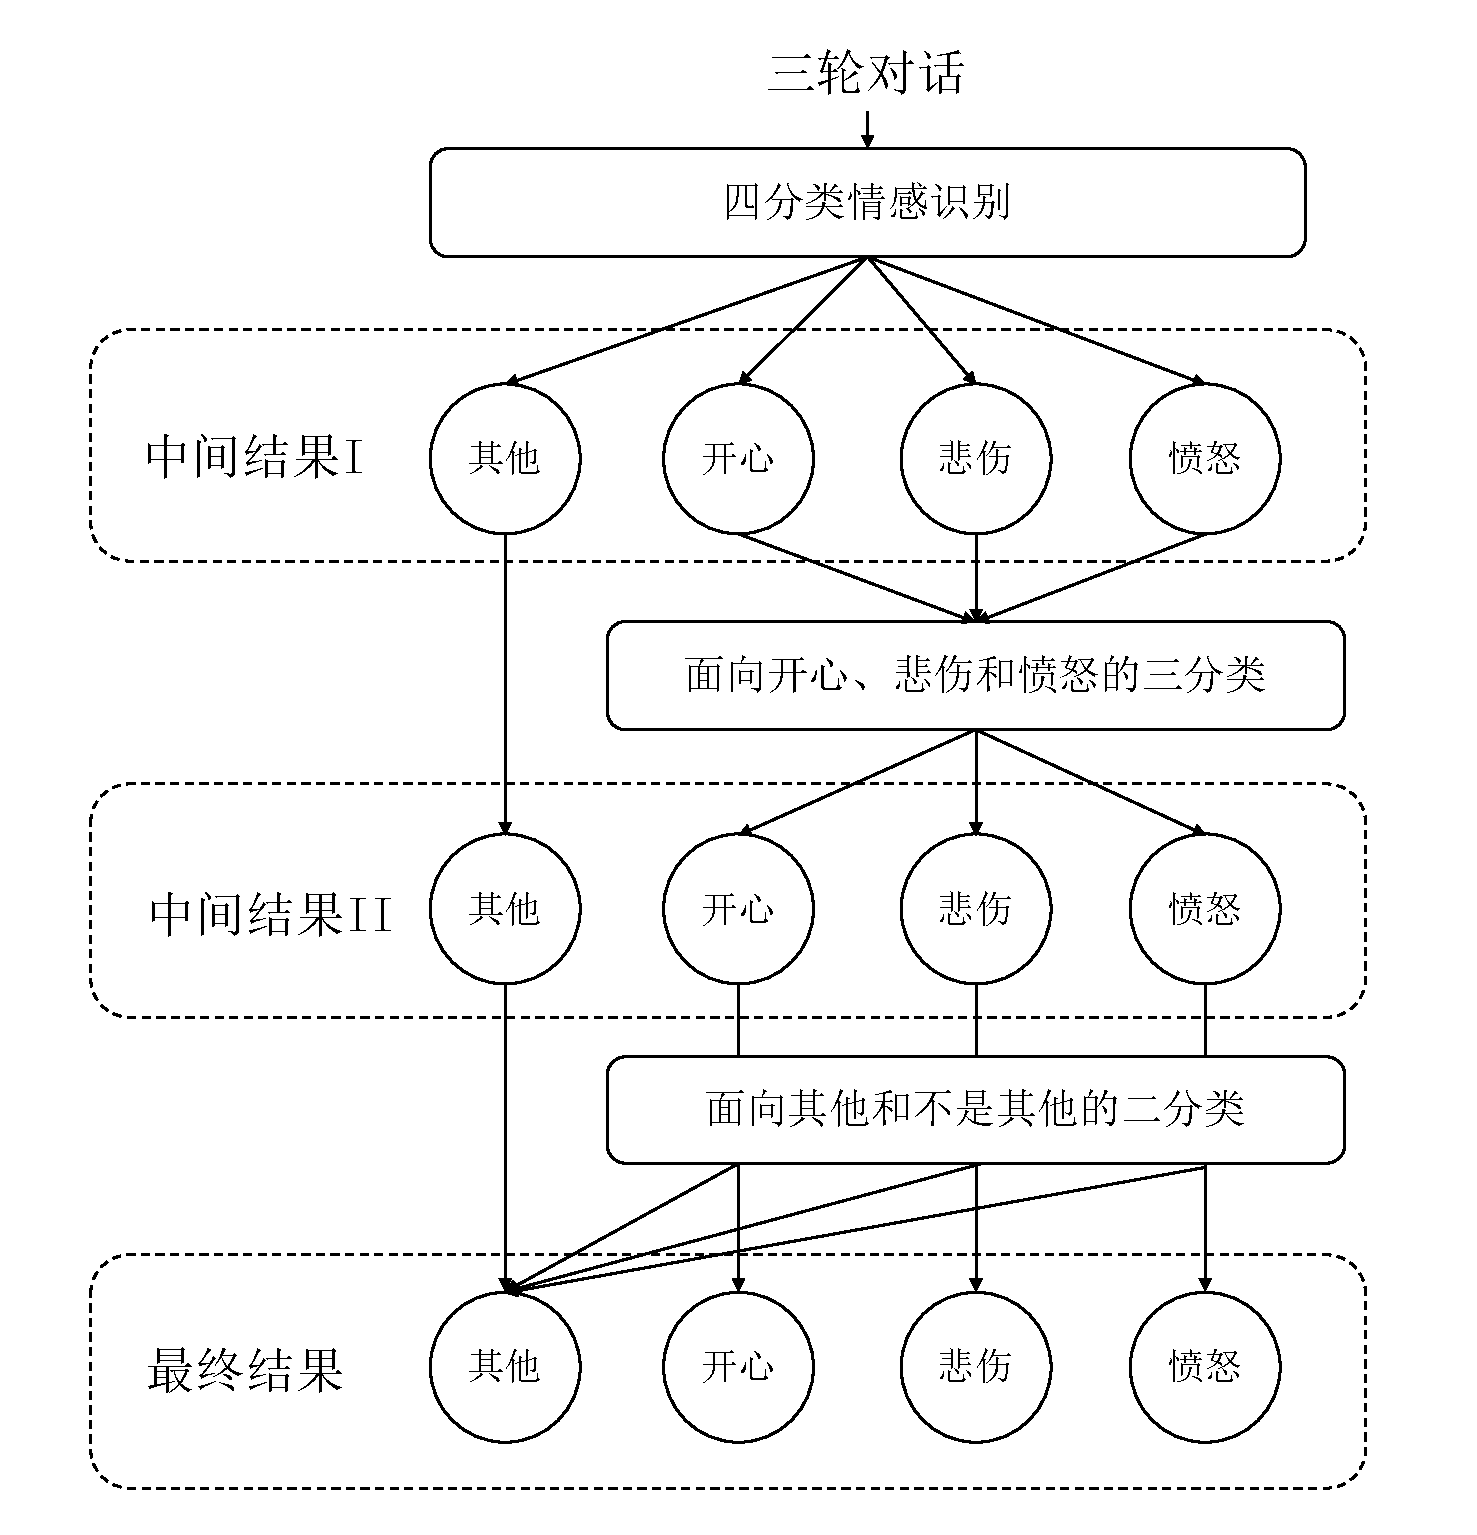
\includegraphics[width=0.9\textwidth]{img/context_emo_system.pdf}
  \caption{三轮对话的情感识别系统框架}
  \label{fig:context_emo_system}
\end{figure}

其中对于每个子分类问题,我们都采用了相同的模型框架,如图\ref{fig:context_emo_cls_framework}所示,每个子分类器的输入为三轮对话对应的词序列$\{w^1, w^2, w^3\}$。根据在章节\ref{ssec:exp_context_emo_multi_turn_analyse}中的分析,我们认为三轮的发言对识别第三轮发言的情感起着不同的作用,因此三轮发言对应的词序列分别进入各自的通道。每个通道的结构相同,第一步都是把词序列转换成对应的词嵌入向量序列,作为特征编码器的输入。此处特征编码器的设计与章节\ref{sec:exp_irony_det_framework}中的相同,目的是把单轮发言对应的词向量序列转换成固定长度的特征向量,以此得出该轮发言的特征向量。为了简化,三个通道的特征编码器采用相同的模型,但考虑到每轮发言的信息中对第三轮情感有关的特征可能不同,故三组模型有各自采用不同的权重。分别得出三轮发言的特征向量后我们需要结合这些特征来预第三轮的情感类别,此处我们直接把三个向量拼接成一个向量,作为概率预测器的轮入。此处概率预测器的设计与章节\ref{sec:exp_irony_det_framework}中的相似,但实现上采用了两层的全联接层,第一层接的激活函数为线性整流函数(Rectified Linear Unit, ReLU),而第二层的激活函数依然为$Softmax$,以得出各个情感类别的概率分布。

同样地,考虑到对于面向不同情感类别的子分类问题,不同模型的建模能力和识别性能可能不同,所以对于每个子分类问题,我们会分别比较各组模型和参数的性能,以求在子分类问题上达到尽可能好的效果。

\begin{figure}[H]
  \centering
  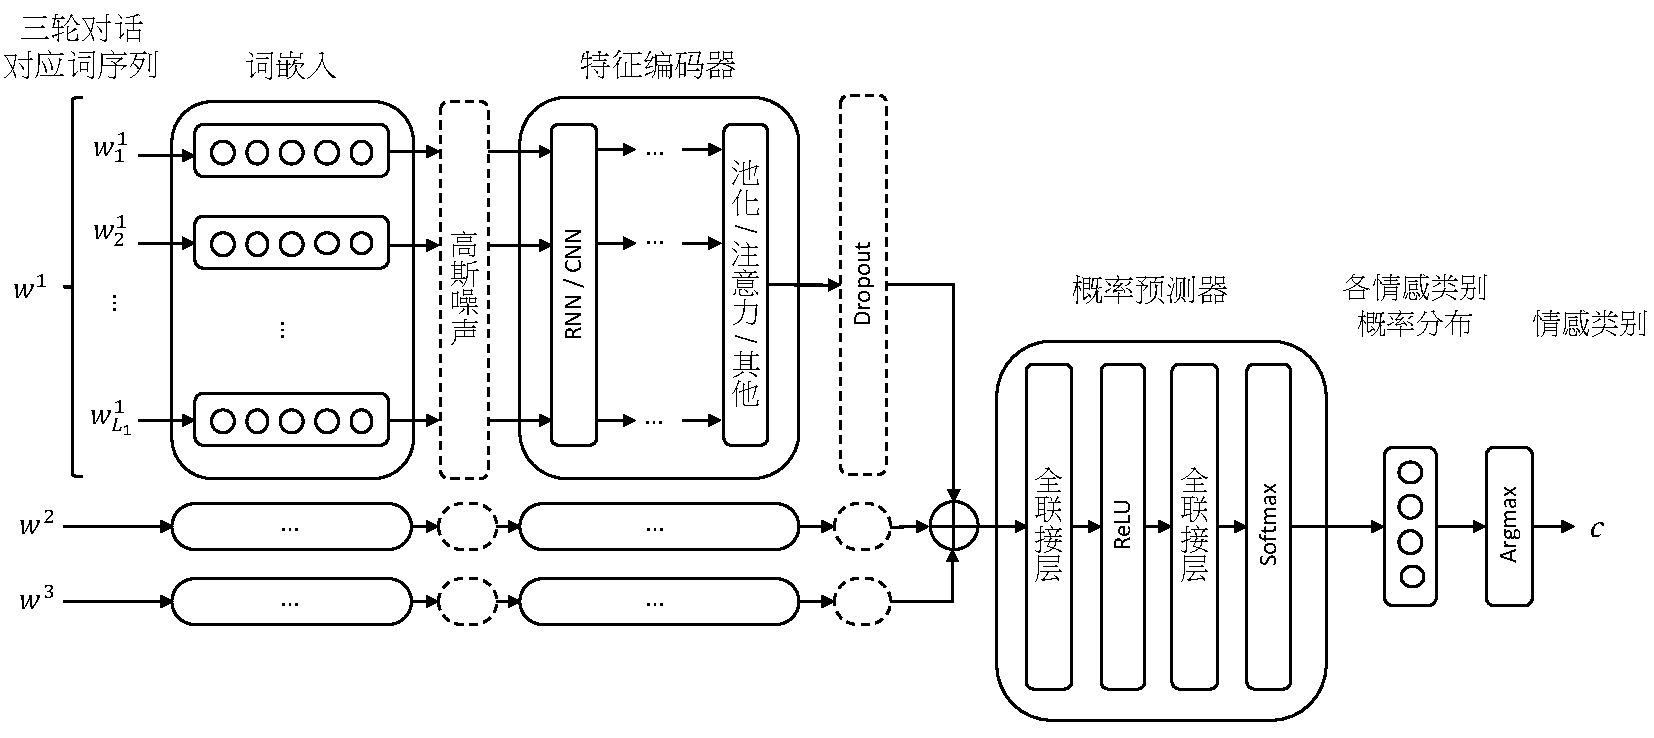
\includegraphics[width=\textwidth]{img/context_emo_cls_framework.pdf}
  \caption{三轮对话的情感识别子分类器模型框架}
  \label{fig:context_emo_cls_framework}
\end{figure}

\section{实验与分析}
\label{sec:exp_context_emo_exp}

\subsection{数据预处理}

基于我们在章节\ref{ssec:exp_context_emo_data_text}中对样本文本的观察,我们依次采取了以下数据预处理手法

\begin{itemize}

\item 全字母大写的内容在前后添加“<allcap>”和“</allcap>”,示意这一段文本可能是用户故意表示强调的内容。

\item 重复大于等次三次的标点符号以“<repeated>”示意,如“!!!”替换成序列“!”和“<repeated>”,表示“!”被多次重复以表达语气加强,同时假设重复次数不影响反讽的类型。

\item 将字母被故意重复的单词以“<elongated>”示意,如“Noooooooo”替换成序列“No”和“<elongated>”,表示“No”中某一个或多个字母被多次重复,但假设被重复的字符和重复的次数与反讽类型无关。

\item 将数字串替换成“<num>”,将电话号码替换成“<phone>”,将日期和时间分别替换成“<date>”和“<time>”,将数字百分比替换成“<percentage>”,超链接替换成“<url>”

\item 将由多个标点符号组成的表情符替换成对应的情感标签,如将“:)”替换成“<happy>”,将“:((”替换成“<sad>”。

\item 在完成以上处理后,对英文的大小写统一转换成小写。

\end{itemize}

\subsection{实验设置}

以下实验主要分成两大部分。第一部分是分析不同模型在不同子分类问题下的性能,根据章节\ref{sec:exp_context_emo_framework},我们最终的反讽识别框架涉及以下多个子分类问题:区分“开心”、“悲伤”、“愤怒”和“其他”的四分类问题,区分“开心”、“悲伤”和“愤怒”的三分类问题、区分“其他”和不是“其他”的二分类问题。对于各个子分类问题,我们基于章节~\ref{sec:exp_context_emo_framework}中的子分类模型框架进行实验,透过采用不同配置了解不同模型对三轮对话的情感识别能力。

第二部分是分析我们设计的识别系统的性能。我们会观察每一轮决策的调整如何改变局部的预测结果,而这些局部变化如何影响系统的整体性能。

\subsection{评价指标}
\label{ssec:exp_context_emo_eval_metric}

按照国际比赛SemEval-2019任务三的设置,系统性能以针对“开心”、“悲伤”和“愤怒”三个情感类别的F1值(以下记为 $F_\mu$)作为识别系统性能的主要评价指标。其定义如下:

\begin{align}
  F_\mu &= \frac{2 \times P_\mu \times R_\mu}{P_\mu + R_\mu}
\end{align}

其中 $P_\mu$ 和 $R_\mu$ 分别是针对“开心”、“悲伤”和“愤怒”三个情感类别的正确率和召回率,其定义如下:

\begin{align}
  P_\mu &= \frac{\sum\limits_{c \in C} TP_c}{\sum\limits_{c \in C}(TP_c + FP_c)} \\
  R_\mu &= \frac{\sum\limits_{c \in C} TP_c}{\sum\limits_{c \in C}(TP_c + FN_c)}
\end{align}

其中 $C$对应情感类别集合\{开心,悲伤,愤怒\},$TP_c$表示被系统预测为类别$c$,且真实标签为类别$c$的样本数量;$FP_c$表示被系统预测为类别$c$,但真实标签不是类别$c$的样本数量;$FN_c$被系统预测为不是类别$c$,但真实标签为类别$c$的样本数量。 

% 同时也关注各个类别各自的F1


\subsection{模型训练}
\label{ssec:exp_context_emo_model_training}

对于不同的模型,我们都采用了以下策略来进行训练:

\begin{itemize}

\item 对于涉及类别“其他”的子分类问题,我们在训练前会基于“其他”的每一个样本随机生成一个新的临时样本(在训练不同子分类器时会各自生成临时样本)。生成方法是在三轮发言中随机选择一轮,再在该轮发言的文本中随机选择一个词删掉,以此摸拟用户使用未被识别的单词或错拼词,得出一个“其他”的新样本。这使得模型对识别“其他”的鲁棒性更好,但同时倾向于将更多不是“其他”的样本识别为“其他”。对于为什么只基于类别“其他”的样本生成新的临时样本,原因在于在语料中,忽略一个单词基本上不影响文本表达“其他”的情感,但对于类别“开心”、“悲伤”和“愤怒”,大部分样本仅由一个或少数几个单词决定其情感属性,若其中的一个单词被忽略会直接导致其情感属性变成中性(即“其他”),为避免产生有误导性的临时样本,我们只基于类别“其他”的样本生成新的样本。

\item 对于每个子分类器,先从每一类的训练样本中随机选出10\%的样本作为验证集,以此保留各个类的样本量分布。在每一轮模型训练中,学习算法基于另外90\%的训练样本对网络参数进行调整,然后计算模型在验证集上的性能,经过有限轮迭代后,取在验证集上某个特定性能指标达到最优的网络参数作为该子分类器最终的参数,以此缓解在训练数据上过拟合的问题。对于第一组分类器(“开心”、“悲伤”、“愤怒”和“其他”四分类)和第二组分类器(“开心”、“悲伤”和“愤怒”三分类),我们采用章节~\ref{ssec:exp_context_emo_eval_metric}中定义的针对“开心”、“悲伤”和“愤怒”的正确率$P_\mu$作为选择参数的性能指标,原因在于人工神经网络对各个类别的识别倾向与训练过程中遇到各类别的样本分布相关(若每个样本在反向传播时的权重相同),而测试集中“开心”、“悲伤”和“愤怒”的样本占比要低于验证集(验证集保留了训练集上各个类别的样本量分布),这导致模型在测试集上较容易把“其他”误判为这三种情感之一,使得正确率$P_\mu$数值明显下降,间接拉低了F1值$F_\mu$,故选择正确率$P_\mu$来确保模型的正确率$P_\mu$尽可能高。而对于第三组分类器(“其他”和不是“其他”二分类),我们采用针对类别“其他”的正确率作为选择参数的性能指标,原因在于对第三组分类器,我们的核心目的是尽可能有信心地召回“其他”的样本,因此要确保单个模型的正确率,而第三组分类器对“其他”样本的召回能力则由分类器的数量弥补。

\item 对于词嵌入层,我们利用了章节\ref{ssec:embedding}中提到的Baziotis等人\cite{baziotis2018ntua}提供的词嵌入模型,直接用于初始化词嵌入层的参数。在训练过程中,我们不对词嵌入层的参数进行调整。另外对于词嵌入模型中未被覆盖的单词,若它在至少2个训练样本中出现,则为其随机生成词向量。原因参考章节\ref{ssec:exp_irony_det_model_training}。

\item 在训练阶段中,我们在词嵌入层后添加高斯噪音。由于词嵌入算法在原理上使得意思相似的单词投影到词嵌入空间中距离相近的点上,高斯噪音的添加相当于把原本的单词替换成近义词,使得模型能更好地识别近义词构成的语言模式,另一方面缓解过拟合的问题。在验证和测试阶段,高斯躁音的标准方差被调整为零,即不起作用。

\item 在训练阶段中,我们在三个通道的特征编码器后分别添加了Dropout层,以概率$p_{Dropout}$将特征编码器得出特征向量上的各位数值置为零,并对没有被置零的各位数值乘以常量 $\frac{1}{1-p_{dropout}}$。在验证和测试阶段,Dropout层不起作用。

\item 在模型训练的损失函数,我们以权重$l_2$加入了概率预测器中两个全联接层的权重(不包括偏移量)的L2正则项。

\end{itemize}

\subsection{结果与分析}

\subsubsection{面向情感四分类的模型性能分析}

对于面向三轮对话的情感四分类问题,表~\ref{tab:exp_context_emo_0_result}和图~\ref{fig:exp_context_emo_0_result_bar}显示不同卷积神经网络和迭归神经网络在我们模型框架中能达到的性能。注意表中的正确率、召回率、F1值为
针对“开心”、“悲伤”和“愤怒”的指示,对应比赛SemEval2019任务三子任务一关注的主要指标,即章节~\ref{ssec:exp_context_emo_eval_metric}中定义的$P_\mu$、$R_\mu$和$F_\mu$。


\begin{table}[htb]
  \centering
  \begin{minipage}[t]{\linewidth}
  \caption{面向情感四分类器的模型性能}
  \label{tab:exp_context_emo_0_result}
    \begin{tabularx}{\linewidth}{X|llll}
    \toprule[1.5pt]
    & 准确率 & 正确率 & 召回率 & F1值 \\
    \hline
    CNN & \bf 0.9245 (1) & 0.7295 (3) & \bf 0.7584 (1) & \bf 0.7437 (1) \\ % f_cnn_ek_1554546621
    CNN+注意力机制 & 0.9071 (5) & 0.6574 (8) & 0.7428 (2) & 0.6975 (3) \\ % f_cnn_ek_1554545828
    \hline
    GRU & 0.9052 (8) & 0.7296 (2) & 0.5481 (9) & 0.6259 (9) \\ % f_gru_ek_1554462561
    GRU+注意力机制 & 0.9105 (3) & \bf 0.7330 (1) & 0.5974 (8) & 0.6583 (7) \\ % f_gru_ek_1554542220
    \hline
    BiGRU & 0.9067 (7) & 0.6598 (7) & 0.6923 (4) & 0.6757 (5) \\ % f_bgru_ek_1554465482
    BiGRU+注意力机制 & 0.9143 (2) & 0.7162 (4) & 0.6947 (3) & 0.7053 (2) \\ % f_bgru_ek_1554524728
    \hline
    LSTM & 0.9071 (5) & 0.6709 (6) & 0.6911 (5) & 0.6809 (4) \\ % f_lstm_ek_1554465719
    LSTM+注意力机制 & 0.8553 (10) & 0.2994 (10) & 0.2788 (10) & 0.2887 (10) \\ % f_lstm_ek_1554560984
    \hline
    BiLSTM & 0.8969 (9) & 0.6331 (9) & 0.6659 (6) & 0.6491 (8) \\ % f_blstm_ek_1554524691
    BiLSTM+注意力机制 & 0.9092 (4) & 0.7067 (5) & 0.6226 (7) & 0.6620 (6) \\ % f_blstm_ek_1554542227
    \bottomrule[1.5pt]
    \end{tabularx}
  \end{minipage}
\end{table}

\begin{figure}[H]
  \centering
  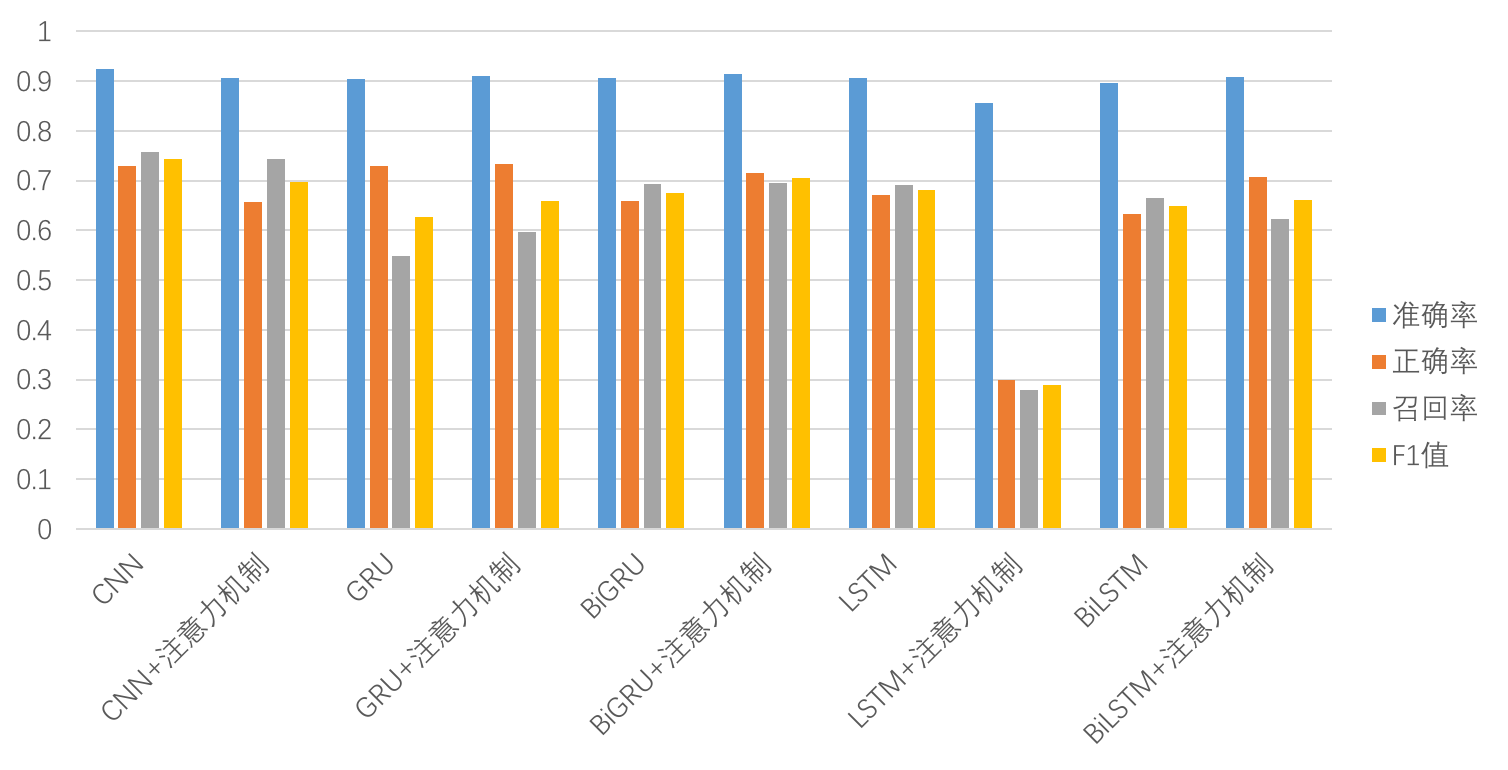
\includegraphics[width=\textwidth]{img/exp_context_emo_0_result_bar.png}
  \caption{面向情感四分类器的模型性能}
  \label{fig:exp_context_emo_0_result_bar}
\end{figure}

\begin{table}[htb]
  \centering
  \begin{minipage}[t]{\linewidth}
  \caption{面向“开心”、“悲伤”和“愤怒”的三分类器模型性能}
  \label{tab:exp_context_emo_b_result}
    \begin{tabularx}{\linewidth}{X|llll}
    \toprule[1.5pt]
    & 准确率 & 正确率 & 召回率 & F1值 \\
    \hline
    CNN & 0.9227 (2) & 0.7202 (2) & 0.7981 (3) & \bf 0.7571 (1) \\ % f_b_cnn_ek_1554620963
    CNN+注意力机制 & 0.9116 (7) & 0.6885 (5) & 0.7572 (9) & 0.7212 (8) \\ % f_b_cnn_ek_1554620537
    \hline
    GRU & 0.9074 (9) & 0.6536 (9) & \bf 0.8233 (1) & 0.7287 (6) \\ % f_b_gru_ek_1554547645
    GRU+注意力机制 & \bf 0.9230 (1) & \bf 0.7434 (1) & 0.7488 (10) & 0.7461 (2) \\ % f_b_gru_ek_1554561028
    \hline
    BiGRU & 0.9134 (4) & 0.6824 (6) & 0.7981 (3) & 0.7357 (4) \\ % f_b_bgru_ek_1554547845
    BiGRU+注意力机制 & 0.9152 (3) & 0.6907 (3) & 0.7945 (6) & 0.7390 (3) \\ % f_b_bgru_ek_1554561013
    \hline
    LSTM & 0.9011 (10) & 0.6347 (10) & 0.8125 (2) & 0.7127 (10) \\ % f_b_lstm_ek_1554549276
    LSTM+注意力机制 & 0.9121 (6) & 0.6895 (4) & 0.7608 (8) & 0.7234 (7) \\ % f_b_lstm_ek_1554554626
    \hline
    BiLSTM & 0.9089 (8) & 0.6708 (8) & 0.7788 (7) & 0.7208 (9) \\ % f_b_blstm_ek_1554549287
    BiLSTM+注意力机制 & 0.9131 (5) & 0.6814 (7) & 0.7969 (5) & 0.7346 (5) \\ % f_b_blstm_ek_1554553473
    \bottomrule[1.5pt]
    \end{tabularx}
  \end{minipage}
\end{table}

\begin{figure}[H]
  \centering
  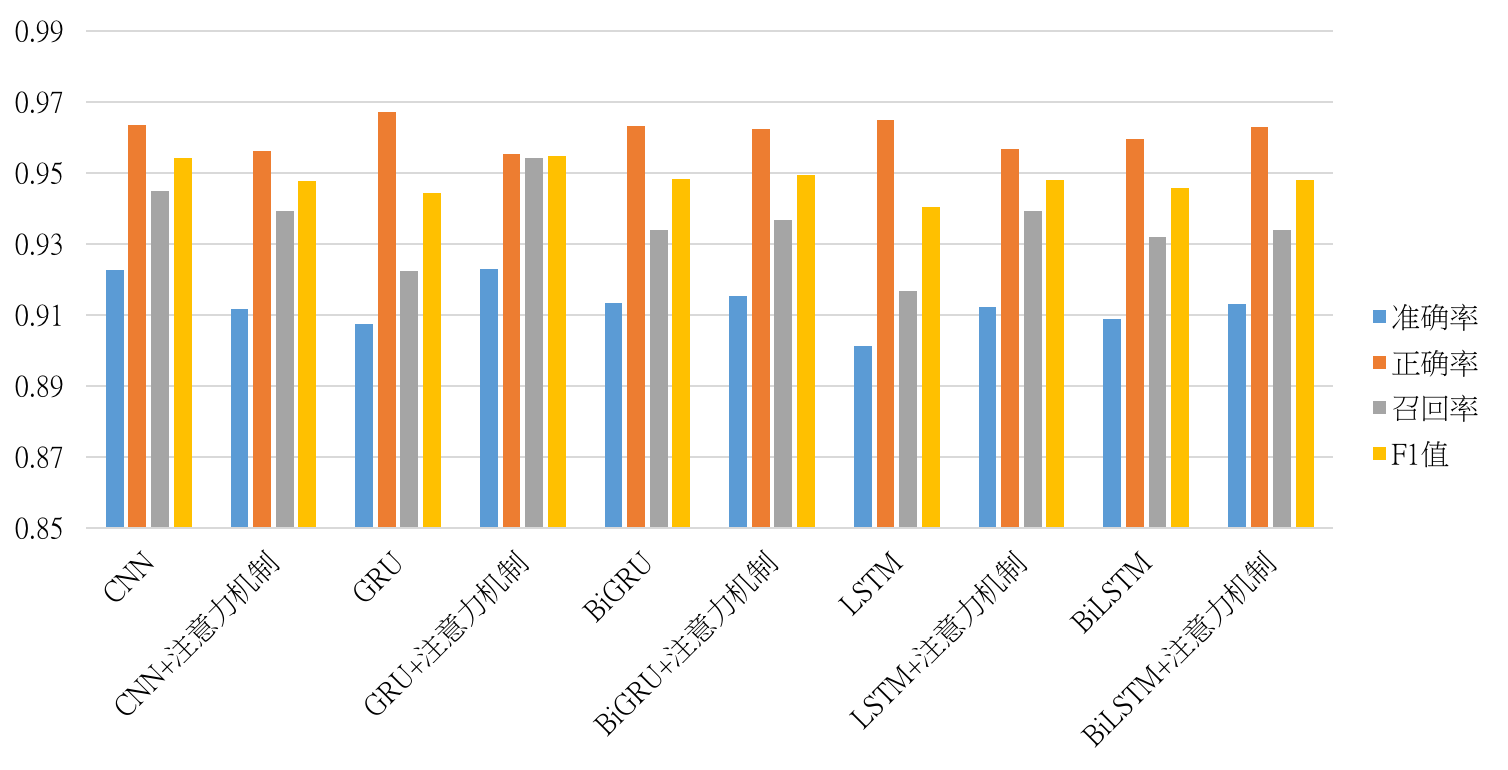
\includegraphics[width=\textwidth]{img/exp_context_emo_b_result_bar.png}
  \caption{面向“开心”、“悲伤”和“愤怒”的三分类器模型性能}
  \label{fig:exp_context_emo_b_result_bar}
\end{figure}

\begin{table}[htb]
  \centering
  \begin{minipage}[t]{\linewidth}
  \caption{面向“其他”和不是“其他”的二分类模型性能}
  \label{tab:exp_context_emo_tri_result}
    \begin{tabularx}{\linewidth}{X|llll}
    \toprule[1.5pt]
    & 准确率 & 正确率 & 召回率 & F1值 \\
    \hline
    CNN & \bf 0.9507 (1) & \bf 0.9454 (1) & \bf 0.9471 (1) & \bf 0.9462 (1) \\ % f_tri_cnn_ek_1554620372
    CNN+注意力机制 & 0.9351 (3) & 0.9352 (2) & 0.9215 (5) & 0.9283 (2) \\ % f_tri_cnn_ek_1554620395
    \hline
    GRU & 0.9315 (6) & 0.9278 (4) & 0.9142 (9) & 0.9210 (6) \\ % f_tri_gru_ek_1554576049
    GRU+注意力机制 & 0.9375 (2) & 0.9303 (3) & 0.9252 (2) & 0.9277 (3) \\ % f_tri_gru_ek_1554612493
    \hline
    BiGRU & 0.9303 (7) & 0.9212 (8) & 0.9179 (7) & 0.9196 (8) \\ % f_tri_bgru_ek_1554576063
    BiGRU+注意力机制 & 0.9339 (4) & 0.9235 (6) & 0.9252 (2) & 0.9243 (5) \\ % f_tri_bgru_ek_1554612494
    \hline
    LSTM & 0.9291 (8) & 0.9229 (7) & 0.9179 (7) & 0.9204 (7) \\ % f_tri_lstm_ek_1554575910
    LSTM+注意力机制 & 0.9279 (9) & 0.9180 (9) & 0.9197 (6) & 0.9189 (9) \\ % f_tri_lstm_ek_1554612497
    \hline
    BiLSTM & 0.9279 (9) & 0.9176 (10) & 0.9142 (9) & 0.9159 (10) \\ % f_tri_blstm_ek_1554575896
    BiLSTM+注意力机制 & 0.9339 (4) & 0.9269 (5) & 0.9252 (2) & 0.9260 (4) \\ % f_tri_blstm_ek_1554612490
    \bottomrule[1.5pt]
    \end{tabularx}
  \end{minipage}
\end{table}

\begin{figure}[H]
  \centering
  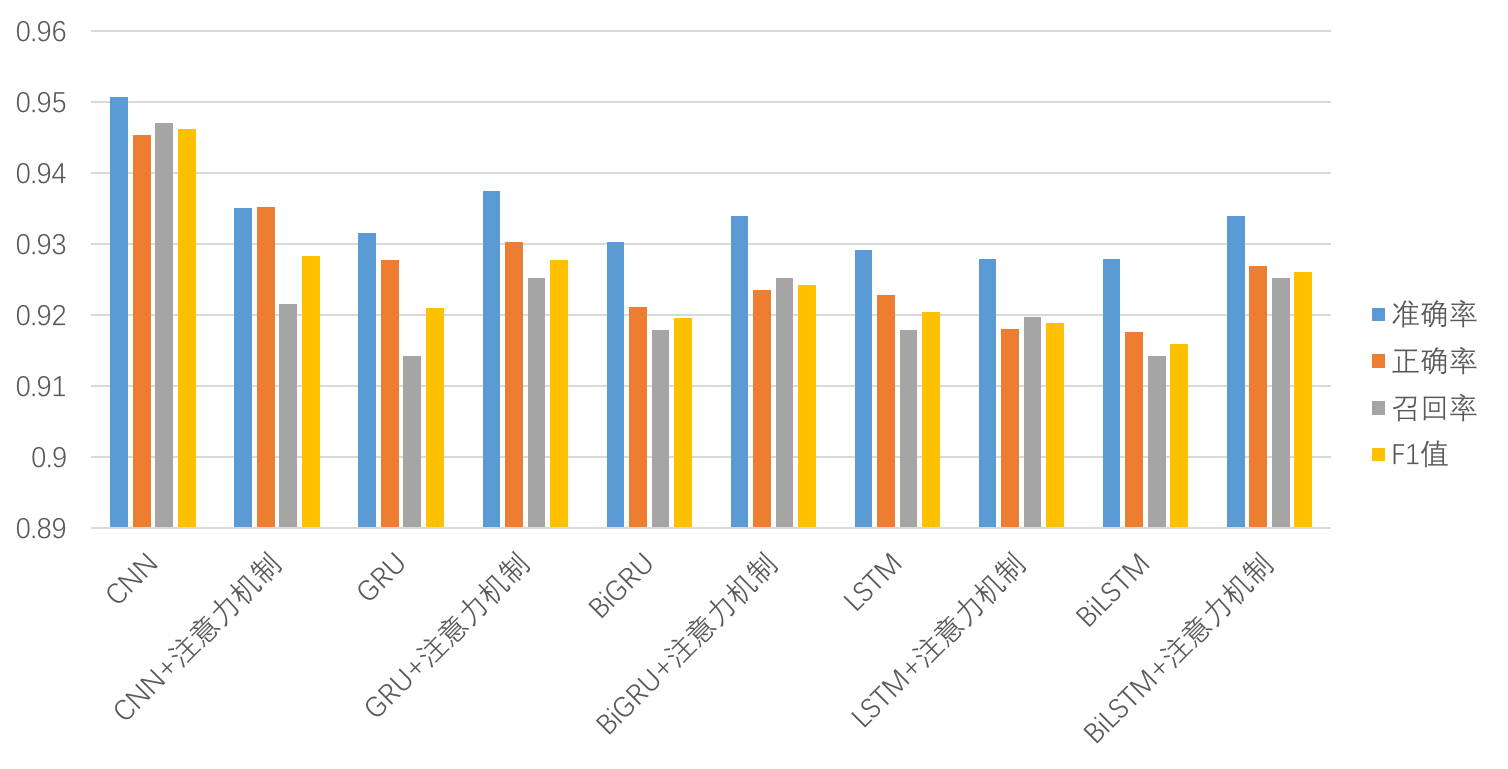
\includegraphics[width=\textwidth]{img/exp_context_emo_tri_result_bar.png}
  \caption{面向“其他”和不是“其他”的二分类模型性能}
  \label{fig:exp_context_emo_tri_result_bar}
\end{figure}

\begin{table}[htb]
  \centering
  \begin{minipage}[t]{0.6\linewidth}
  \caption{多步决策后的系统识别性能}
  \label{tab:exp_context_emo_ensemble_result}
    \begin{tabularx}{\linewidth}{X|cccc}
    \toprule[1.5pt]
    & 准确率 & 正确率 & 召回率 & F1值 \\
    \hline
    中间结果I & 0.9278 & 0.7360 & 0.7740 & 0.7545 \\
    中间结果II & 0.9281 & 0.7383 & \bf 0.7764 & 0.7569 \\
    \hline
    最终结果 & \bf 0.9305 & \bf 0.7553 & 0.7680 & \bf 0.7616 \\ 
    \bottomrule[1.5pt]
    \end{tabularx}
  \end{minipage}
\end{table}

\begin{table}[htb]
  \centering
  \begin{minipage}[t]{0.6\linewidth}
  \caption{SemEval-2019任务三前十名参赛系统性能} % 总参赛队伍165
  \label{tab:exp_context_emo_other_comp}
    \begin{tabularx}{\linewidth}{c|X|c}
    \toprule[1.5pt]
    排名 & 队伍名称 & F1值 \\
    \hline
    1 & PingAn GammaLab & 0.7959 \\
    2 & (无) & 0.7947 \\
    3 & NELEC & 0.7765 \\
    4 & SymantoResearch & 0.7731 \\
    5 & ANA & 0.7709 \\
    6 & CAiRE\_HKUST & 0.7677 \\
    7 & SNU\_IDS & 0.7661 \\
    8 & \bf THU\_HCSI & 0.7616 \\
    9 & (无) & 0.7608 \\
    10 & YUN-HPCC & 0.7588 \\
    \bottomrule[1.5pt]
    \end{tabularx}
  \end{minipage}
\end{table}



\section{本章小结}

pass

